\centerline{19.03.2025}


\centerline{\bf \large Региональный этап XVII  республиканской математической олимпиады}
\centerline{\bf \large  школьников  имени академика РАО  П.М. Эрдниева  }

\centerline{\bf \Large  9 класс}

\problem{\textbf{1}} 
Пюрвя загадал число, которое имеет $2025$ различных делителей, отличных от $1$ и самого числа. Сколько простых делителей может быть у числа Пюрви?


\problem{\textbf{2}} Решите задачу:

а) Батыр и Очир ходили вокруг школы, оба в одном направлении и каждый с постоянной скоростью. Батыр проходил один круг за 5 минут, а Очир, который был медленнее Батыра, - за некоторое целое число минут. При этом время между встречами тоже равнялось некоторому целому числу минут, причём оно было больше 12. За какое время Очир проходил полный круг?

б) Составьте и решите обратную задачу по схеме: ?; 6; 12.


\problem{\textbf{3}} Прямая проходит через точку с координатами $(2025 ; 0)$ и пересекает параболу $y=$ $x^2$ в точках с абсциссами $a$ и $b$. Найдите $\dfrac{1}{a}+\dfrac{1}{b}$.


\problem{\textbf{4}} 
Дан вписанный четырёхугольник $A B C D$. Прямые $A B$ и $D C$ пересекаются в точке $E$, а прямые $B C$ и $A D$ - в точке $F$. В треугольнике $A E D$ отмечен центр вписанной окружности $I$, а из точки $F$ проведен луч, перпендикулярный биссектрисе угла $A I D$. В каком отношении этот луч делит угол $A F B$ ?

\problem{\textbf{5}}
На координатной плоскости назовём \textit{бриллиантовым расстоянием} между двумя точками $A$ и $B$, находящимися в узлах, количество клеток, которые пересекает отрезок $AB$. Также назовём \textit{бриллиантовым кругом} радиуса $n$ геометрическое место точек, удалённых от данной на бриллиантовое расстояние $n$. Докажите, что бриллиантовый круг радиуса $n$ с центром в начале координат совпадает со множеством узлов сетки, заданных уравнением $|x| + |y| = n+1$, где $x,y$ - целые тогда и только тогда, когда $n+1$ простое.

\centerline{\bf }


\centerline{\bf  Желаем удачи!}
\centerline{\bf  Время на выполнение 240 минут.}

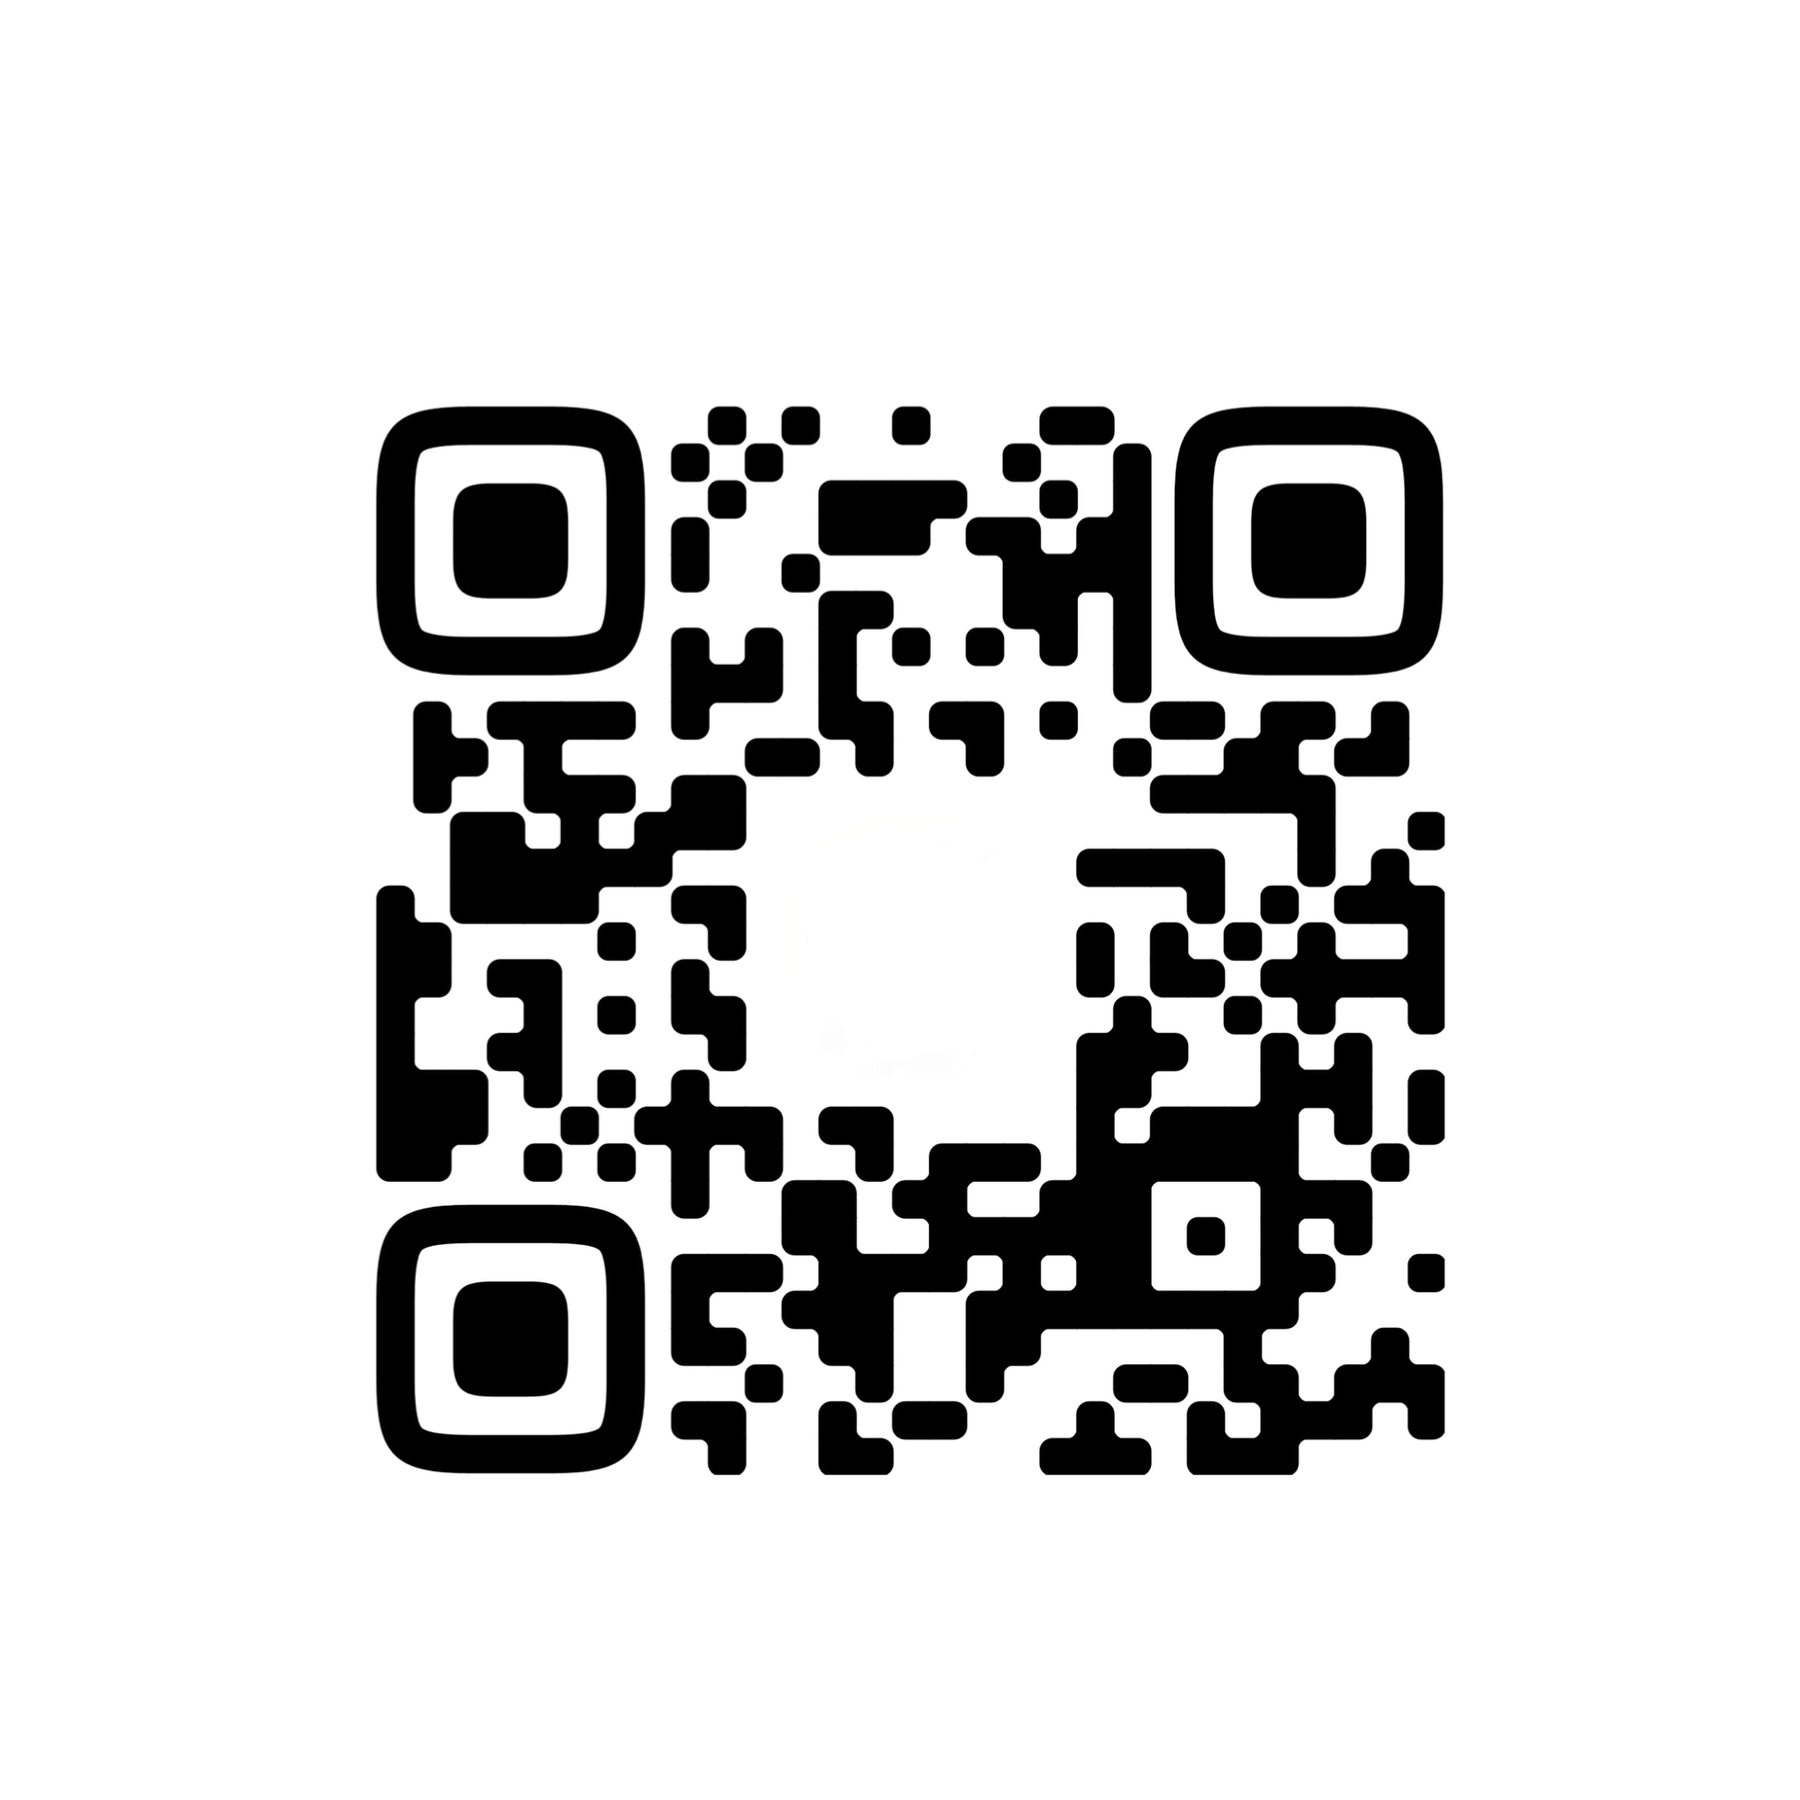
\includegraphics[width=5cm]{Секретная информация/УДЕ 2024-2025/QR_code.jpg} % Левая картинка
    \hfill
    \textbf{Разбор в 15:00 по QR - коду слева.}
    \hfill

\includegraphics[width=5cm]{Секретная информация/УДЕ 2024-2025/logo_ude.png} % Правая картинка